\documentclass[11pt,a4paper]{article}
\usepackage[utf8]{inputenc}
\usepackage[T1]{fontenc}
\usepackage{amsfonts}
\usepackage[french]{babel}
\frenchbsetup{StandardLists=true} % à inclure si on utilise \usepackage[francais]{babel}
\usepackage{enumitem}
\usepackage{amssymb}
\usepackage{amsmath}
\usepackage[left=2cm,right=2cm,top=2cm,bottom=2cm]{geometry}
\usepackage{multirow}
\usepackage[dvipsnames]{xcolor}

\usepackage[T1]{fontenc}
\usepackage{fouriernc}
\usepackage{graphicx}

\usepackage{setspace}
\singlespacing

\usepackage{multicol}
\usepackage{caption}
\usepackage{fancyhdr}
\pagestyle{fancy}
\renewcommand\headrulewidth{1pt}
\fancyhead[L]{Lycée Denis Diderot }
\fancyhead[R]{Classe de Terminale}
\setcounter{page}{10}\fancyfoot[C]{page \thepage}
\fancyfoot[R]{Année 2025 2026}
\fancyfoot[L]{Alexis RUIZ}
\usepackage{multirow,tabularx,booktabs}
\newcommand{\cadreblanc}[1]{%
\medskip\framebox[\linewidth][c]{%
\rule{0mm}{#1mm}}\par
\medskip}

\renewcommand{\arraystretch}{2}
\newcommand*\acocher{\quitvmode{\fboxsep0pt \fboxrule0.8pt \fbox{\vrule height1.8ex depth.1ex width0pt \vrule height0pt depth0pt width1.9ex }}}

\begin{document}
\center \LARGE{TP3 - Pont de diodes}
\\[0,3cm]

\normalsize

\hrule\
\\[0,2cm]

\flushleft \textbf{NOM :\\
Prénom:\\[0,2cm]
}
\hrule\
\\[0,2cm]

\fbox{MONTAGE 1} Réaliser le montage ci-dessous en utilisant les réglages suivants : \\
\begin{itemize}
\item tension alternative de 6 V;
\item au moins 2 périodes visualisables sur l'oscilloscope;
\item l'amplitude sur l'écran la plus grande possible.
\end{itemize}

\begin{center}
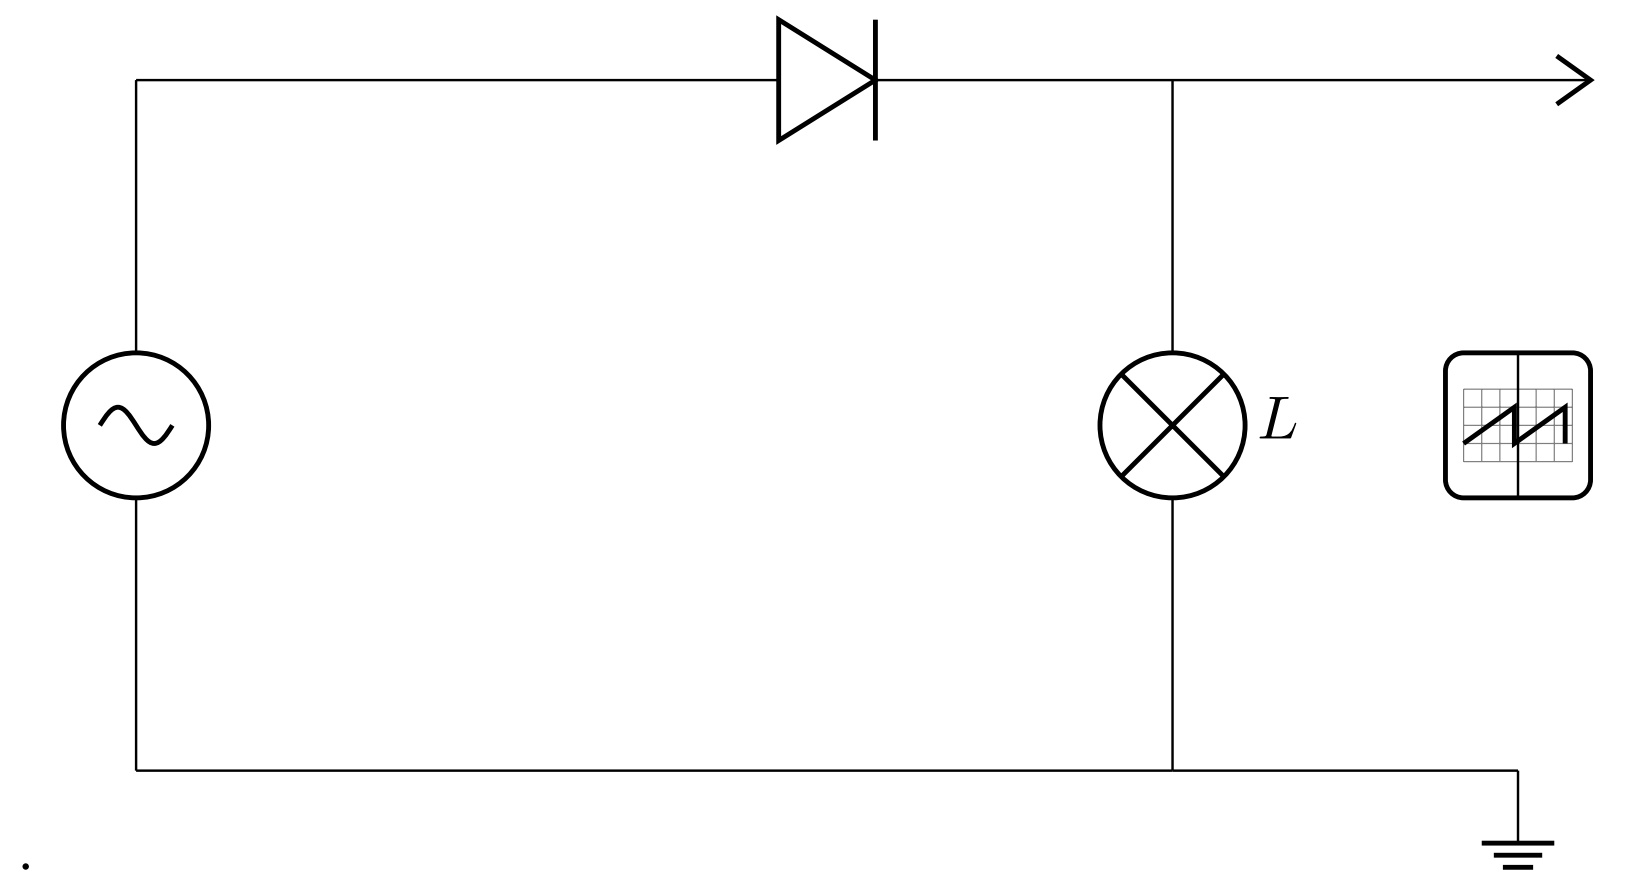
\includegraphics[scale=0.3]{images/montage 1.png} 



\includegraphics[scale=0.25]{images/appel exam.png}\\   Appeler M Ruiz\\
\hrule\
\\[0,2cm]

\renewcommand{\arraystretch}{2.8}
\begin{tabularx}{12 cm}{|c||X|X|}
\hline
Évaluation & Montage & Réglages\\

\hline 


 
\end{tabularx}
\end{center}

\dotfill\\

\begin{center}\textbf{Tester les 3 autres diodes}\\
\end{center}

\hrule
\begin{center}
Représenter l'oscillogramme obtenu à l'écran de l'oscilloscope.
\end{center}


\begin{multicols}{2}
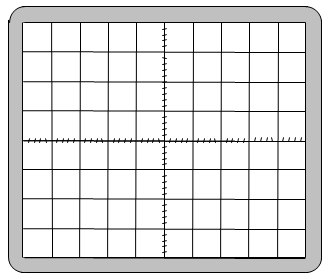
\includegraphics[scale=0.6]{images/ecran oscillo.png} 



\renewcommand{\arraystretch}{2.8}
\begin{tabularx}{8 cm}{|c||X|X|}
\hline
Valeurs & $U_{Max}=$ & $T=$\\
\hline 
\end{tabularx}

\renewcommand{\arraystretch}{2.8}
\begin{tabularx}{8 cm}{|c||X|X|}
\hline
Calculs & $U_{Eff}=$ & $f=$\\
\hline 
\end{tabularx}

\end{multicols}
La tension observée est-elle alternative ? Justifier votre réponse
\cadreblanc{20}



\newpage

\fbox{MONTAGE 2} Réaliser le montage ci-dessous en utilisant les réglages suivants : \\
\begin{itemize}
\item tension alternative de 6 V;
\item au moins 2 périodes visualisables sur l'oscilloscope;
\item l'amplitude sur l'écran la plus grande possible.
\end{itemize}
\begin{center}
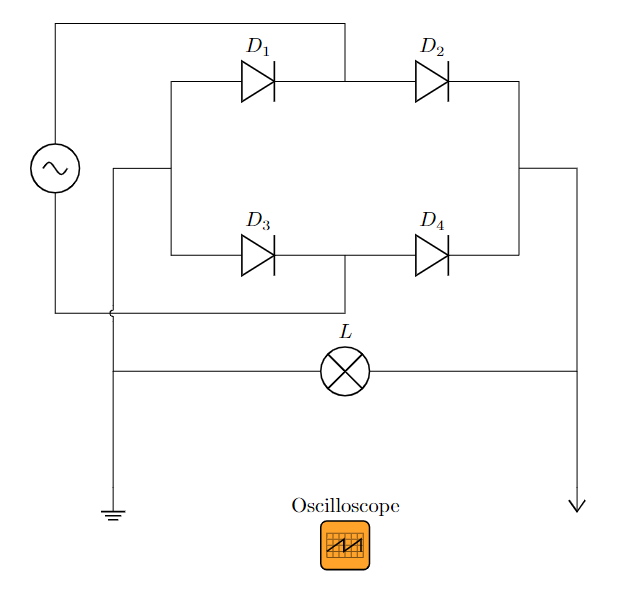
\includegraphics[scale=0.65]{images/Pont de diodes ss C.png} 


\includegraphics[scale=0.5]{images/appel exam.png}\\   Appeler M Ruiz\\

\renewcommand{\arraystretch}{2.8}
\begin{tabularx}{12 cm}{|c||X|X|}
\hline
Évaluation & Montage & Réglages\\
\hline 


 
\end{tabularx}
\end{center}

\begin{center}
Représenter l'oscillogramme obtenu à l'écran de l'oscilloscope.
\end{center}


\begin{multicols}{2}
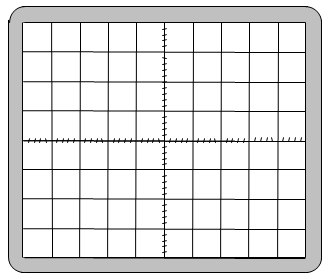
\includegraphics[scale=0.7]{images/ecran oscillo.png} 



\renewcommand{\arraystretch}{2.8}
\begin{tabularx}{8 cm}{|c||X|X|}
\hline
Valeurs & $U_{Max}=$ & $T=$\\
\hline 
\end{tabularx}

\renewcommand{\arraystretch}{2.8}
\begin{tabularx}{8 cm}{|c||X|X|}
\hline
Calculs & $U_{Eff}=$ & $f=$\\
\hline 
\end{tabularx}
\\[6mm]
Quel est le rôle du pont  de diodes ? 
\cadreblanc{25}
\end{multicols}



\newpage

\fbox{MONTAGE 3} Réaliser le montage ci-dessous en utilisant les réglages suivants : \\
\begin{itemize}
\item tension alternative de 6 V;
\item l'amplitude sur l'écran la plus grande possible.
\end{itemize}

\begin{center}
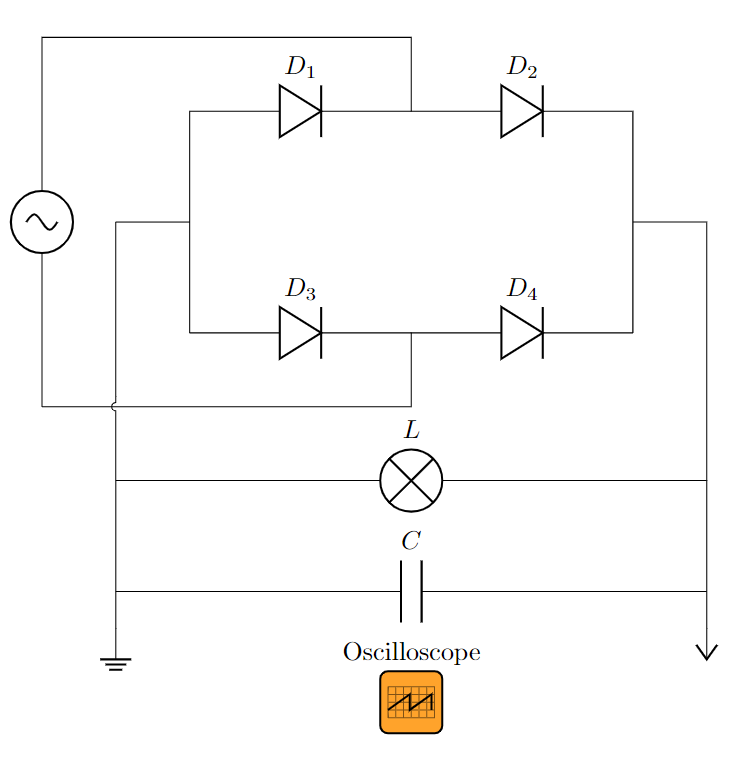
\includegraphics[scale=0.5]{images/Montage - Pont.png} 


\includegraphics[scale=0.5]{images/appel exam.png}\\   Appeler M Ruiz\\

\renewcommand{\arraystretch}{2.8}
\begin{tabularx}{12 cm}{|c||X|X|}
\hline
Evaluation & Montage & Réglages\\
\hline 
 
\end{tabularx}
\end{center}


\begin{multicols}{2}
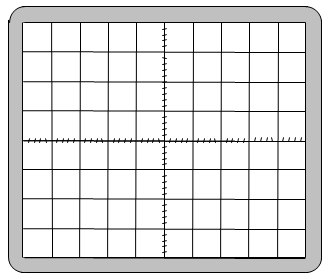
\includegraphics[scale=0.65]{images/ecran oscillo.png} 
Déterminer la valeur de la tension en V :\\
\cadreblanc {15}
De quel type de tension s'agit-il ? 
\cadreblanc{20}

\end{multicols}




Quel est le rôle du condensateur ? 
\cadreblanc{25}


\end{document}